A análise de regressão é um conjunto de métodos estatísticos que buscam ajustar uma função preditora de uma variável resposta com base em uma ou mais variáveis explicativas.

Seja $X$ uma variável explicativa e $Y$ uma variável resposta. Para cada $X$, deseja-se estimar a distribuição condicional de $Y | X$, conforme ilustrado na Figura \ref{fig:exemplo_regressao}.

\begin{figure}[H]
    \centering
    \caption{Dispersão de pontos com distribuições de $Y | X$}
    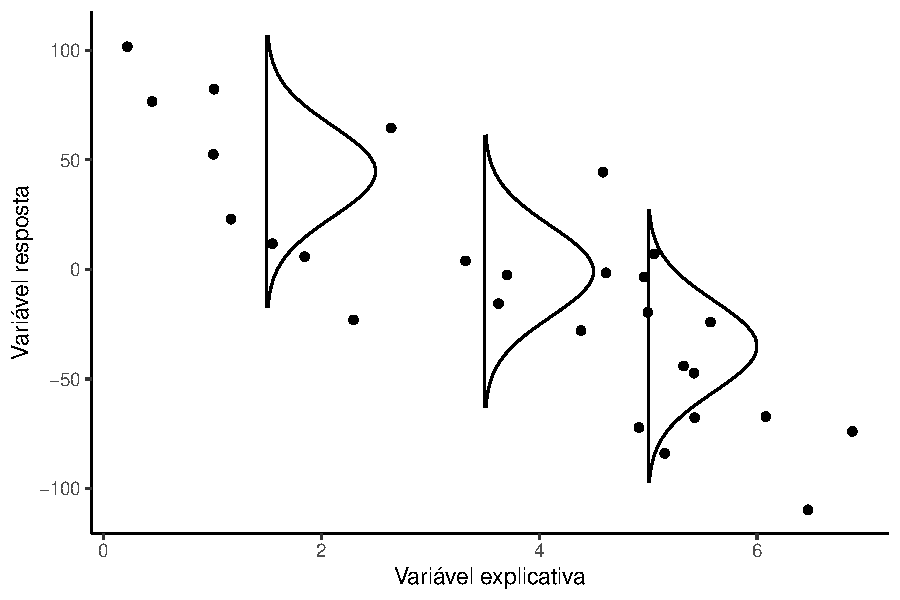
\includegraphics[scale=1.05]{imagens/scatter2.pdf}
    \label{fig:exemplo_regressao}
\end{figure}

 Os dois métodos que serão utilizados no trabalho, cujos resultados serão comparados entre eles, são a regressão gaussiana e a regressão quantílica, que estimam, respectivamente, a média condicional $E(Y|X)$ e os quantis condicionais $Q(Y|X)_\tau$.

\subsection{Regressão Gaussiana}
A regressão gaussiana linear, ou regressão tradicional, é um método que ajusta uma reta que minimiza a diferença quadrática entre um conjunto de pontos e a média observada.

Há cinco pressupostos principais para um modelo de regressão gaussiana:

\begin{enumerate}
    \item A correlação entre a média condicional E(Y|X) da variável resposta e as variáveis explicativas é linear, ou seja, descrita por uma combinação linear entre as variáveis explicativas e os parâmetros do modelo.
    \item Os erros $\varepsilon_i$ tem média $\mu = 0$.
    \item Os erros $\varepsilon_i$ tem variância constante $\sigma^2$.
    \item Os erros $\varepsilon_i$ são não-correlacionados entre eles.
    \item Os erros possuem distribuição Normal.
\end{enumerate}

Seja $\mathbf{x}$ um vetor de variáveis aleatórias independentes e $\varepsilon$ um vetor de erros aleatórios, onde $\varepsilon$ satisfaz a propriedade de ser Normalmente distribuído, com média $\mu = 0$ e variância $\sigma_i ^ 2$ constante para cada $\varepsilon_i$, qualquer que seja o valor de $x_i$ ($i \in \{1, \dots, n\}$). Seja $Y$ uma variável resposta. A regressão gaussiana ajusta um vetor de coeficientes $\beta$ de uma equação
\begin{equation}
Y = \beta ^ {T} \mathbf{x} + \varepsilon,
\end{equation}

\noindent minimizando a soma dos quadrados dos erros, e prediz o valor médio de $Y$ condicionado aos valores de $\mathbf{x}$.

É possível demonstrar que, satisfeitos os pressupostos do modelo, o vetor de coeficientes $\beta$ pode ser estimado na forma

\begin{equation}
\hat{\beta} = (\mathbf{X}^{T}\mathbf{X})^{-1} \mathbf{X}^{T} \mathbf{y},
\end{equation}

\noindent onde $\mathbf{X}$ é a matriz de valores observados ordenados das variáveis explicativas, e $\mathbf{y}$ é o vetor de valores observados da variável resposta $Y$ \cite{montgomerylra}.

\newpage
\subsection{Regressão Quantílica}
No que se refere aos pressupostos, a regressão quantílica é menos restritiva do que o modelo gaussiano, pois não assume Normalidade dos erros, tampouco homoscedasticidade. A regressão quantílica assume que os erros são não-correlacionados entre eles e $Q_\tau(\varepsilon_\tau | x) = 0$.

Embora modelos quantílicos não-lineares também sejam possíveis, este projeto assumirá que as relações entre as variáveis são lineares.

Diferente do modelo de regressão gaussiana, que traça a reta para a média de uma variável resposta dependente de variáveis explicativas, a regressão quantílica traça a reta para qualquer quantil selecionado. Isso a torna mais robusta que o modelo de mínimos quadrados no que se refere à influência de outliers. Assim, é possível obter análises mais ricas sobre o fenômeno estudado, expandindo a funcionalidade clássica dos modelos de regressão.

O $\tau$-ésimo quantil de uma distribuição de probabilidades é qualquer ponto $y$ da variável aleatória tal que a probabilidade de um valor ser menor ou igual a $y$ é igual a $\tau$. Pela definição, considerando $F(y)$ a função de distribuição acumulada da variável aleatória $y$, temos que

\begin{equation}
\tau = P(Y \leq y) = F(y).
\end{equation}

No caso empírico, com probabilidades zeradas no intervalo entre duas observações, convenciona-se o uso do valor mínimo do intervalo, de modo que a definição para o quantil assume a forma
\begin{equation}
F^{-1}(\tau) = \text{inf}\{y: F(y) \geq \tau\}.
\end{equation}

A distribuição empírica permite reduzir a estimativa para o quantil segundo métodos de otimização da função de perda

\begin{equation}
\rho_\tau(u) = u(\tau - I(u < 0)), \tau \in (0, 1),
\end{equation}

\noindent onde $I(u < 0)$ é uma função indicadora que assume valor 1 se $u < 0$ e valor 0, caso contrário. Os métodos de otimização podem ser implementados computacionalmente com programação linear. Assim, encontra-se o $\hat{x}$ que minimiza

\begin{equation}
\displaystyle \min_{\xi \in \mathbb{R}} \displaystyle \sum_{i=1}^{n} \rho_\tau(y_i - \xi).
\end{equation}

Analogamente, podemos reduzir o problema da regressão quantílica a um problema de otimização de uma distribuição condicional. Segue que o resultado deve resolver

\begin{equation}
\displaystyle \min_{\beta \in \mathbb{R}^{p}} \displaystyle \sum_{i=1}^{n} \rho_\tau(y_i - x_i^{\text{T}}\beta).
\end{equation}


Seja $Q_\tau(Y | X)$ a função de quantil condicional, com Y sendo uma variável aleatória dependente e X conhecido. Seja $\beta$ um vetor de funções de $\tau$ que multiplicam as variáveis explicativas. É possível demonstrar que, resolvido o problema de otimização, obtém-se uma expressão da forma

\begin{equation}
Q_\tau(Y | X) = \beta_0(\tau) + x_1 \beta_1(\tau) + \dots + x_n \beta_n(\tau)  = {\beta} (\tau) \mathbf{x}
\end{equation}

\noindent onde cada $x_{i}$, com $i \in \{1, ..., n\}$, é uma variável explicativa, e $Q_\tau(Y | X)$ é o quantil condicional $\tau$ de $Y$ dado $X$  \cite{koenker2005}.

Se a variação do $\beta(\tau)$ for pequena em função de $\tau$, significa que os erros são identicamente distribuídos, tornando a abordagem de regressão quantílica desnecessária, uma vez que a mesma solução poderia ser modelada a partir de uma regressão linear clássica usando menos recurso computacional. A abordagem quantílica, portanto, se torna faz mais necessária em casos heteroscedásticos, com os quais a regressão linear não teria seus pressupostos satisfeitos.

\subsubsection{Intervalos de confiança para os coeficientes do modelo de regressão quantílica}
A construção de intervalos de confiança será utilizada na 